\documentclass[10pt,landscape]{article}

%encoding
\usepackage[T1]{fontenc}
\usepackage[utf8]{inputenc}
\usepackage{lmodern}

%language
\usepackage[english]{babel}

%paper and text body handling
\usepackage{geometry}
\usepackage{setspace}
\usepackage{lettrine}

%graphics
\usepackage{graphicx}
\usepackage[format = plain, labelfont = {bf, it}, textfont = it]{caption}%font settings for captions
\usepackage{xcolor}
\usepackage{pdfpages}
\usepackage{subcaption}
\usepackage{tcolorbox}
\usepackage{multicol}
\usepackage{tikz}
\usetikzlibrary{arrows.meta}
\usetikzlibrary{bending}


%code
%\usepackage{minted}

%math
\usepackage{amsmath}%math
\usepackage{amssymb}%
\usepackage{amsfonts}%
\usepackage{amsthm}%theorems
\usepackage{aligned-overset}
\usepackage{siunitx}
\usepackage{cancel}
\usepackage{braket}
\usepackage{bm}
\usepackage{diffcoeff}
\usepackage{bbold}
% Use the correct ds in diffs
\diffdef{}{
  op-symbol = \mathrm{d},
  op-order-sep = 0 mu
}

%links
\usepackage[colorlinks=true,
            linkcolor=red,
            urlcolor=blue,
            citecolor=gray]{hyperref}


% Specific to this paper
\newcommand{\maj}{\succ}
\newcommand{\majby}{\prec}
%special letters
\newcommand{\R}{\mathbb{R}}
\newcommand{\C}{\mathbb{C}}
\newcommand{\Z}{\mathbb{Z}}
\newcommand{\N}{\mathbb{N}}
\newcommand{\F}{\mathcal{F}}
\newcommand{\PP}{\mathbb{P}}
\newcommand{\EE}{\mathbb{E}}
\newcommand{\idty}{\mathbb{1}}

%functions
\renewcommand{\Re}{\textnormal{Re}}
\renewcommand{\Im}{\textnormal{Im}}
\DeclareMathOperator{\Var}{Var} % Variance
\DeclareMathOperator{\Cov}{Cov} % Covariance
\DeclareMathOperator{\Res}{Res} % Residue
\DeclareMathOperator{\Ker}{Ker} % Kernel
\DeclareMathOperator{\tr}{tr} 	% Trace
\newcommand{\scalprod}[2]{\left\langle#1, #2\right\rangle}

\DeclarePairedDelimiter\abs{\lvert}{\rvert}%
\DeclarePairedDelimiter\norm{\lVert}{\rVert}%

% Swap the definition of \abs* and \norm*, so that \abs
% and \norm resizes the size of the brackets, and the
% starred versions do not.
\makeatletter
\let\oldabs\abs
\def\abs{\@ifstar{\oldabs}{\oldabs*}}
%
\let\oldnorm\norm
\def\norm{\@ifstar{\oldnorm}{\oldnorm*}}
\makeatother

%symbols
% for := as
\newcommand*{\defeq}{%
    \mathrel{%
        \vcenter{%
            \baselineskip0.5ex \lineskiplimit0pt \hbox{\scriptsize.}\hbox{\scriptsize.}%
        }%
    }%
    =%
}


%settings

%spacing
\renewcommand{\arraystretch}{1.2}
\setlength{\arraycolsep}{3pt}

%units
\sisetup{
   output-decimal-marker = {,},
   exponent-product = \ensuremath{\cdot}
}

%text
\makeatletter
   \newlength{\textSize}
   \setlength{\textSize}{\f@size pt}
\makeatother
\setlength{\parindent}{0pt}             % No indentation on new paragraph
%\setstretch{1.15}


%paper and text body
\geometry{
	top=0.5cm,
	bottom=0.5cm,
	left=0.5cm,
	right=0.5cm,
   a4paper,
   centering,
}


%lettrine settings
\setcounter{DefaultLines}{3}


\newcommand{\topiccolor}{green}
\newcommand{\topic}[2]{%
	\renewcommand{\topiccolor}{#1}
	\begin{tcolorbox}[boxsep=0.5mm, left=1mm, right=1mm, top=0mm, bottom=0mm,
		colback=#1!30, colframe=#1, arc is angular]%
		\centering \textbf{#2}%
	\end{tcolorbox}%
}
\newcommand{\cbf}[1]{\textcolor{\topiccolor!70!black}{\textbf{#1}}}

\begin{document}

\begin{multicols*}{3}
\begin{tcolorbox}[colframe=black, colback=white]
	\centering \large Computational Quantum Mechanics
\end{tcolorbox}

\topic{blue}{One-body problem}

For time-independent 1D SE, we use \cbf{the Numerov algorithm}.
It solves $f''(x) = k(x)f(x)$.
To do this, Taylor expand $f$ and add $f(x+\Delta x) + f(x-\Delta x)$.
In that expression, replace the fourth derivative by the finite difference
approximation to the second derivative of $f''$, and $f''$ by $k(x)f(x)$.
To get started, you thus need two points, $\Delta x$ apart.
Bound states can be found using the \cbf{Bidirectional-Shooting method}.
Perform Numerov from right and left and scale them so they match.
Vary $b$ until the derivatives match too.
\begin{center}
	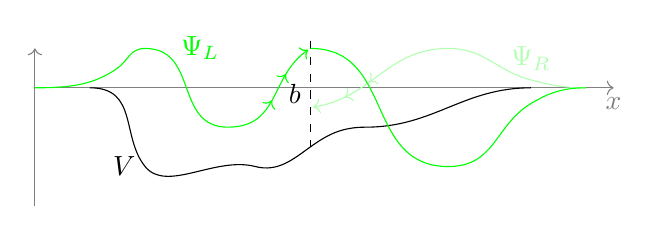
\begin{tikzpicture}[xscale=0.7, yscale=0.5]
		% Coordinate axes
		\draw[->,gray] (0, -3) -- (0, 1);
		\draw[->,gray] (0,0) -- (10.5,0) node[anchor=north]{$x$};
		% Potential
		\draw (1, 0) to[out=0, in=120] (2, -2) node[anchor=east]{$V$}
					 to[out=300, in=160] (4,-2)
					 to[out=-20, in=225] (5,-1.5)
					 to[out=45, in=180] (6,-1)
					 to[out=0, in=180] (9,0);
		% b
		\draw[dashed] (5,1.2) -- node[anchor=east]{$b$} (5,-1.5);
		% non-continuous
		\draw[out=0, in=180, color=\topiccolor,
			-{>[sep=10pt]>[sep=10pt]>[sep=1pt]}]
			(0,0) to[in=225] (1.5,0.5)
				  to[out=45] (2,1) node[xshift=0.7cm]{$\Psi_L$}
				  to (3.5,-1)
				  to[in=220] (5, 1);
		\draw[out=180, in=0, color=\topiccolor!30,
			-{>[sep=10pt]>[sep=10pt]>[sep=1pt]}]
			(10,0) to[in=-20] (9,0.2) node[anchor=south]{$\Psi_R$}
				   to[out=160] (7.5,1)
				   to[in=10] (5,-0.5);
		% Continuous
		\draw[out=180, in=0, color=\topiccolor,]
			(10,0) to[in=40] (9,-0.4)
				   to[out=-140] (7.5,-2)
				   to (5,1)[in=-20];

	\end{tikzpicture}
\end{center}

For higher dimensions, try using symmetries first because partial differential
equation solvers are a lot more difficult to handle. Try factorizing
$\psi(\mathbf{r}) = \psi_x(x)\psi_y(y)\psi_z(z)$. Or if the potential has a
spherical symmetry, try an ansatz with the spherical harmonics.

For solving the time-\emph{dependent} Schrödinger equation, we either use
spectral methods -- expressing the initial wave function as a linear combination
of energy eigenfunctions and evolving those -- but this is only tractable for
small systems since we need an eigenbasis. The other method is direct numerical
integration for which we use the \cbf{split operator method}.
\[
	e^{-i\Delta t(\hat T + \hat V)} \approx 
	e^{-i \Delta t \hat V / 2} e^{-i \Delta t \hat T} e^{-i \Delta t \hat V / 2}
\]
for small $\Delta t$.

\topic{cyan}{Matrix Product States / Operators}

No thank you!

\topic{red}{Monte-Carlo methods}

\cbf{MC integration}:
$\int f(x) \dl x = \sum_{x_i} f(x_i)/N$.

\cbf{Importance sampling}:
$\int f(x) \dl x = \int f(x)/p(x) \cdot p(x) \dl x = \sum_{x_i} f(x_i) / p(x_i)$,
$x_i$ sampled from pdf $p(x)$.

\cbf{MCMC}: $x_i$ generated from Markov Chain
For $x_i$ to be distributed as $p(x)$, it is sufficient that
\cbf{detailed balance} is fulfilled:
\[
	T(x \to x') p(x) = T(x' \to x) p(x')
\]
For the \cbf{metropolis method}, $T(x \to x') = \omega_{xx'}A_{x x'}$,
where $\omega$ is a symmetric, stochastic matrix which should
be interpreted as a proposal distribution and $A_{x x'}$ is
to be treated as acceptance probabilities.

The \cbf{Wolff algorithm} can be useful when simulating the Ising model
using MCMC.
It proposes new states where entire clusters of spins are flipped,
instead of just one.

We can also use MCMC for \cbf{quantum spin systems}. To do so, we must use a
quantum to classical mapping:
\[
	Z = \tr\left[e^{-\beta \hat H}\right]
	= \sum_C W(C)
\]%
\[
	\braket{\hat m} = \tr\left[\hat m e^{-\beta \hat H} \right]
	= \sum_C m(C) W(C)
\]
It turns out that we can always make a mapping from a d-dimensional quantum
system to a (d+1)-dimensional classical system.
For a single spin-1/2 you can accomplish it by splitting the exponential into a
product of $M$ factors and inserting a resolution of identity between all of
them:
\[
	Z = \sum_i \braket{i | U^M |i}
	= \sum_{\{i_1,\ldots,i_M\}} \braket{i_1|U|i_2}\bra{i_2}
	\cdots\ket{i_M}\braket{i_M|U|i_1}
\]
Increasing $M$ to infinity, the probability of having two neighbouring sites
with opposite spin goes to 0 at a rate such that the total number of domain
walls remains finite. Therefore, we can change our description to only keep
track of where the domain walls are.
\begin{center}
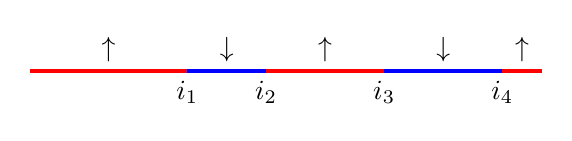
\begin{tikzpicture}
	\draw (0,0) -- node[anchor=south]{$\uparrow$}
		(2,0) node[anchor=north]{$i_1$} [color=red, ultra thick];
	\draw (2,0) -- node[anchor=south]{$\downarrow$}
		(3,0) node[anchor=north]{$i_2$} [color=blue, ultra thick];
	\draw (3,0) -- node[anchor=south]{$\uparrow$}
		(4.5,0) node[anchor=north]{$i_3$} [color=red, ultra thick];
	\draw (4.5,0) -- node[anchor=south]{$\downarrow$}
		(6,0) node[anchor=north]{$i_4$} [color=blue, ultra thick];
	\draw (6,0) -- node[anchor=south]{$\uparrow$}
		(6.5,0) [color=red, ultra thick];
\end{tikzpicture}
\end{center}
\cbf{Quantum Monte Carlo for particles} is yet another application of MC methods
this time to $N$ quantum particles in $d$ dimensions in a thermal state.
Do again subdivision into $M$ factors and resolution of identity, though this
time with $\int \ket{R}\bra{R} \dl R$.
This gives a high dimensional integral which we calculate with MCMC methods.
The configuration being sampled is the many-particle paths.
Updates are proposed by choosing a single time slice of a single world line (a
\cbf{bead}) and moving it a bit (gaussian proposal).
\begin{center}
	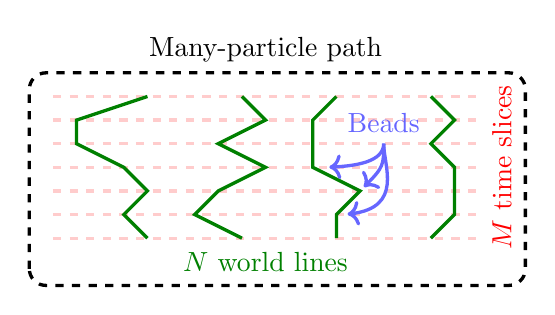
\begin{tikzpicture}[scale=0.3, very thick]
		% Time slices
		\foreach \y in {0,...,6}
			\draw (-4, \y) -- (14, \y) [dashed, color=red!20];

		% World lines
		\draw (0,0) -- (-1,1) -- (0,2) -- (-1,3) -- (-3,4) -- (-3,5) -- (0,6)
			[color=green!50!black];
		\draw (4,0) -- (2,1) -- (3,2) -- (5,3) -- (3,4) -- (5,5) -- (4,6)
			[color=green!50!black];
		\draw (8,0) -- (8,1) -- (9,2)  -- (7,3) -- (7,4) -- (7,5) -- (8,6)
			[color=green!50!black];
		\draw (12,0) -- (13,1) -- (13,2) -- (13,3) -- (12,4) -- (13,5) -- (12,6)
			[color=green!50!black];

		\draw [<-, blue!60, shorten <=2pt] (9,2) .. controls (10,3) .. (10,4)
			node[anchor=south]{Beads};
		\draw [<-, blue!60, shorten <=6pt] (7,3) .. controls (8,3) and (10,3) .. (10,4);
		\draw [<-, blue!60, shorten <=4pt] (8,1) .. controls (11,1) and (10,3) .. (10,4);
		\node at (15, 3) [rotate=90, color=red] {$M$ time slices};
		\node at (5, -1) [color=green!50!black] {$N$ world lines};
		\node at (5, 8) []{Many-particle path};
		\draw [dashed, rounded corners=6pt] (-5, -2) rectangle  (16, 7);
	\end{tikzpicture}
\end{center}
The goal of \cbf{Diffusion Monte Carlo} is to find the ground state of a bosonic
system.
Instead of fixing $\beta$ and splitting it into $\Delta \tau M$ and wiggling the
world lines, we fix $\tau$ and apply $e^{-\Delta\tau \hat H}$ a bunch of times.
The state is $M$ walkers with positions and weights (initially random/1).
Applying the operator consists of drawing displacements from a gaussian,
which incorporates the kinetic energy part of $\hat H$, and updating the weights
using the potential. We then remove walkers with low weights and add copies of
ones with high weights. This is an alternative method to the acceptance
probability previously discussed.

\topic{orange}{Electronic structure}

How do we find the energy eigenstates of a molecule?
The relevant Hamiltonian is
\[
	\begin{split}
		H &= 
		-\sum_j^{N_e} \frac{\hbar^2}{2m_e} \nabla^2_{r_j} 
		- \sum_\ell^{N_n} \frac{\hbar^2}{2m_\ell} \nabla^2_{R_\ell}
		+ \frac12 \sum_{i\neq j} \frac{e^2}{\abs{r_i - r_j}}\\
		  &\phantom{=} 
		+ \frac12 \sum_{\ell\neq m} \frac{Z_\ell Z_m e^2}{\abs{R_\ell - R_m}}
		- \sum_{j,\ell}^{N_e, N_n} \frac{Z_\ell e^2}{\abs{r_j - R_\ell }}\\
		  &= T_e + T_n + V_{ee} + V_{nn} + V_{ne}
	\end{split}
\]
The first step is to use the \cbf{Born-Oppenheimer Approximation}:
nuclei are heavy compared to electrons, so they're effectively frozen when
solving for the electron wave functions.

The \cbf{Hartree} method is assuming non-interacting electrons in a mean field.
You first guess some wavefunctions for the individual electrons and then,
using these as the wavefunction the electrons interact with,
calculate new wavefunctions and iterate until it seems to converge.
Once converged, take a slater determinant to find the ground state.

The \cbf{Hartree-Fock} method also assumes non-interacting
electrons in a mean field, but the asymmetry is considered from the beginning.
First take some orthonormal set of single-electron wave functions $\phi_i$.
Then take some new single-electron wave functions that are linear combinations
of these: $\varphi_k = \sum_i \alpha_{ik} \phi_i$.
Letting $\Psi$ be the many body wave function gotten from a Slater determinant
of the $\varphi_k$, minimize $\braket{\Psi | H_\text{BO} | \Psi}$.
Writing it out gives rise to an \emph{exchange term} owing to the Pauli
principle.

\cbf{Density Functional Theory} is concerned with the electron ground state
density $n_0$, rather than the actual wavefunction. 
There is a one-to-one correspondence between $n_0$ and $V_\text{ext}$.
In the case of molecules, $V_\text{ext} = V_{ne}$, but we could have a more
general external potential.
The clever point is that everything that is not $V_\text{ext}$ is the same no
matter which system we are trying to solve.
The energy functional that we minimize is
\begin{align*}
	E_{[v_\text{ext}]}[n] &= \min_{\Psi\to n} 
	\braket{\Psi| T_e + V_{ee} + V_\text{ext} |\Psi}\\
	&= \min_{\Psi\to n} 
\braket{\Psi| T_e + V_{ee} |\Psi}
	+ \int \dl r v_\text{ext}(r) n(r)
\end{align*}
The first term we call $F[n]$ and that is universal -- it does not depend on the
specific problem. The $\Psi \to n$ notation means $\Psi$ such that the density is
$n$.

Unfortunately, since the correlations in $\Psi$ can be complicated (i.e.\ it is
not a single Slater determinant state), this is still not an easy
problem. The \cbf{Kohn-Sham solution scheme} tries to remedy this by trying to
find a non-interacting (i.e. it \emph{is} a single Slater determinant state)
system with the same density as the exact one.
To compensate for the errors coming from this ignoring of the correlation,
we add an additional term including the unknown correction called the
exchange-correlation functional $E_{XC}$:
\[
	E[n] = E_k[n] + E_c[n] + E_{XC}[n] + V_\text{ext}[n]
\]
Minimizing this under the condition $\int n \dl n = N_e$ using lagrange
multipliers gives single-particle equations called the Kohn-Sham equations.
\begin{align*}
	\left[-\frac{\hbar^2}{2 m_e} \nabla^2 + V_\text{eff}(r)\right] \varphi_j =
	\varepsilon_j \varphi_j\\
	V_\text{eff}(r) = \int \dl r' \frac{n}{\abs{r - r'}} + V_{XC}(r) +
	V_\text{ext}(r)
\end{align*}
Note that this is in principle just a trick to find the density, you should not
expect the single particle energies $\varepsilon_j$ to actually correspond to
the single particle energies of the system.


\end{multicols*}

\end{document}
